\documentclass[a4paper,14pt]{extarticle}

\usepackage[utf8x]{inputenc}
\usepackage[T1]{fontenc}
\usepackage[russian]{babel}
\usepackage{hyperref}
\usepackage{indentfirst}
\usepackage{here}
\usepackage{array}
\usepackage{graphicx}
\usepackage{grffile}
\usepackage{caption}
\usepackage{subcaption}
\usepackage{chngcntr}
\usepackage{amsmath}
\usepackage{amssymb}
\usepackage[left=2cm,right=2cm,top=2cm,bottom=2cm,bindingoffset=0cm]{geometry}
\usepackage{multicol}
\usepackage{multirow}
\usepackage{titlesec}
\usepackage{listings}
\usepackage{listingsutf8}
\usepackage{color}
\usepackage{enumitem}
\usepackage{cmap}
\usepackage{titlesec}

\definecolor{green}{rgb}{0,0.6,0}
\definecolor{gray}{rgb}{0.5,0.5,0.5}
\definecolor{purple}{rgb}{0.58,0,0.82}

\lstdefinelanguage{none}{}

\lstset{
	language={C++},
	inputpath={../},
	backgroundcolor=\color{white},
	commentstyle=\color{green},
	keywordstyle=\color{blue},
	numberstyle=\color{gray}\scriptsize\ttfamily,
	stringstyle=\color{purple},
	basicstyle=\lst@ifdisplaystyle\footnotesize\fi\ttfamily,
	breakatwhitespace=false,
	breaklines=true,
	captionpos=b,
	keepspaces=true,
	numbers=left,
	numbersep=5pt,
	showspaces=false,
	showstringspaces=false,
	showtabs=false,
	tabsize=4,
	frame=single,
	morekeywords={NULL, DWORD, WINAPI, HANDLE, STARTUPINFO, BYTE, LPSTR, SOCKET, WSADATA, TCHAR, LPCTSTR, LPOVERLAPPED, WSABUF, SECURITY_ATTRIBUTES, SECURITY_DESCRIPTOR, TRUE, FALSE, PROCESS_INFORMATION, PIPE_UNLIMITED_INSTANCES, LPVOID, sockaddr_in},
	deletekeywords={error},
	alsoletter={_},
	sensitive=true,
	extendedchars=false,
	columns=fullflexible,
	inputencoding=utf8/cp1251,
	literate=%
		{~}{{\raise.25ex\hbox{$\mathtt{\sim}$}}}{1}%
		{-}{-}{1}
}

\makeatletter
\def\lst@outputspace{{\ }}
\makeatother

\renewcommand{\le}{\ensuremath{\leqslant}}
\renewcommand{\leq}{\ensuremath{\leqslant}}
\renewcommand{\ge}{\ensuremath{\geqslant}}
\renewcommand{\geq}{\ensuremath{\geqslant}}
\renewcommand{\epsilon}{\ensuremath{\varepsilon}}
\renewcommand{\phi}{\ensuremath{\varphi}}
\renewcommand{\thefigure}{\arabic{figure}}
\newcommand{\code}[1]{\lstinline|#1|}
\newcommand{\caret}{\^{}}
\newcommand{\ctrl}[1]{\^{}{#1}}
\newcommand{\listingwithoutput}[1]{
	\lstinputlisting[caption=\code{#1.cpp}]{src/#1/#1.cpp}
	Выполним программу \code{#1.exe}:
	\lstinputlisting[language=none]{logs/#1/#1.txt}
}

\titleformat*{\section}{\large\bfseries}
\titleformat*{\subsection}{\normalsize\bfseries}
\titleformat*{\subsubsection}{\normalsize\bfseries}
\titleformat*{\paragraph}{\normalsize\bfseries}
\titleformat*{\subparagraph}{\normalsize\bfseries}

\titlespacing{\section}{0em}{0.8em}{0.8em}

\counterwithin{figure}{section}
\counterwithin{equation}{section}
\counterwithin{table}{section}
\newcommand{\sign}[1][5cm]{\makebox[#1]{\hrulefill}}
\newcommand{\equipollence}{\quad\Leftrightarrow\quad}
\newcommand{\no}[1]{\overline{#1}}
\graphicspath{{../pics/}}
\captionsetup{justification=centering,margin=1cm}
\def\arraystretch{1.3}
\setlength\parindent{5ex}
\titlelabel{\thetitle.\quad}

\setitemize{topsep=0em, itemsep=0em}
\setenumerate{topsep=0em, itemsep=0em}

\begin{document}

\begin{titlepage}
\begin{center}
	Санкт-Петербургский Политехнический Университет Петра Великого\\[0.3cm]
	Институт компьютерных наук и технологий \\[0.3cm]
	Кафедра компьютерных систем и программных технологий\\[4cm]
	
	\textbf{ОТЧЕТ}\\ 
	\textbf{по лабораторной работе}\\[0.5cm]
	\textbf{<<Процессы и потоки в Windows>>}\\[0.1cm]
	Операционные системы\\[3.0cm]
\end{center}

\begin{flushright}
	\begin{minipage}{0.5\textwidth}
		\textbf{Работу выполнил студент}\\[3mm]
		группа 43501/3 \hfill Дьячков В.В.\\[5mm]
		\textbf{Работу принял преподаватель}\\[5mm]
		\sign[2cm] \hfill к.т.н., доц. Душутина Е.В. \\[5mm]
	\end{minipage}
\end{flushright}

\vfill

\begin{center}
	Санкт-Петербург\\[0.3cm]
	\the\year
\end{center}
\end{titlepage}

\addtocounter{page}{1}

\tableofcontents
\newpage

\section{Цели работы}

Изучение систем отладки и структурированной обработки исключений в ОС Windows.

\section{Программа работы}

\renewcommand{\labelenumii}{\theenumii}
\renewcommand{\theenumii}{\theenumi.\arabic{enumii}.}

\textbf{Порождение и запуск процессов}

\begin{enumerate}
	\item Неименованные каналы (pipe):
		\begin{enumerate}
			\item Создать клиент-серверное приложение, позволяющее набираемые символы в терминальном окне командной строки (сервер) отображать их в окно процесса-потомка (клиент).
			\item Создать эхо-сервер, взаимодействующий с клиентом посредством pipe.
		\end{enumerate}
	\item Именованные каналы (named pipe):
		\begin{enumerate}
			\item Реализовать между одним клиентом и сервером обмен данными, вводимыми с консоли на стороне клиента и возвращаемыми сервером обратно до получения команды exit.
			\item Реализовать между сервером и множеством клиентов обмен данными, вводимыми с консоли на стороне клиента и возвращаемыми сервером обратно до получения команды exit.
			\item Модифицировать приложение из предыдущего примера для сетевого обмена информацией.
		\end{enumerate}
	\item Сокеты (socket):
		\begin{enumerate}
			\item Реализовать программ локального и сетевую обмена с помощью сокетов с использованием потокового протокола с установлением соединения (TCP в стеке TCP/IP).
			\item Модифицировать программу для локального обмена с множеством клиентов и с доступом к общему ресурсу. Провести эксперимент с множеством клиентов при сетевом обмене, представить результаты для виртуальной и реальной сетей.
			\item Проанализировать пример применения сокетов (сетевой обмен «мгновенными» сообщениями).
			\item Привести примеры использования портов завершения. Привести пример приложения с большим количеством клиентов до 1000 (когда порты завершения оправданы), общее количество потоков не более 10.
			\item Реализовать обмен на основе UDP.
		\end{enumerate}
	\item Сигналы (signal):
		\begin{enumerate}
			\item Задать обработчик сигналов завершения для консольного приложения.
			\item Самостоятельно предложить собственную реализацию обработчика сигнала.
		\end{enumerate}
	\item Разделяемая память (file mapping):
		\begin{enumerate}
			\item Создать программу, в которой первый процесс генерирует случайное число и записывает его в буфер, доступный второму процессу, откуда он его и считывает с последующим выводом.
		\end{enumerate}
	\item Почтовые слоты (MailSlot):
		\begin{enumerate}
			\item Предложить собственную реализацию приложения, иллюстрирующую обмен информацией почтовыми слотами. Продемонстрировать возможность локального и удаленного доступа. Выполнить широковещательную передачу данных.
		\end{enumerate}
\end{enumerate}

\section{Используемое окружение}

\begin{itemize}
	\item ОС: Windows 10 Pro
	\item Версия ОС: 1803 (сборка 17134.1069)
	\item Процессор: Intel® Core™ i7-8550U CPU @ 1.80GHz × 8
	\item ОЗУ: 16 Гб
	\item Компилятор: MSVC 14.23.28105, C/C++ Optimizing Compiler Version 19.23.28105.4 for x64
\end{itemize}

\section{Структурированная обработка исключений}

\subsection{Исключение}

Структурированная обработка исключений (SEH -- Structured Exception Handling) -- механизм обработки программных и аппаратных исключений в операционной системе Microsoft Windows, позволяющий программистам контролировать обработку исключений.

Исключение -- это событие при выполнении программы, которое приводит к её ненормальному или неправильному поведению. Существует два вида исключений: аппаратные, которые генерируются процессором, и программные, генерируемые операционной системой и прикладными программами. Механизм структурной обработки исключений позволяет однотипно обрабатывать как программные, так и аппаратные исключения.

Исключение может быть continuable или non-continuable. Non-continuable исключение возникает в том случае, когда событие является непрерывным в аппаратном обеспечении, и его продолжение не имеет смысла. Такое исключение не завершает работу приложения; таким образом, исключение может быть обработано. Однако non-continuable исключение обычно возникает в результате повреждения стека или другой серьезной проблемы, что затрудняет восстановление после исключения.

\subsection{Основные функции и структуры для работы с SEH}

\begin{itemize}
	\item \cpp{DWORD GetExceptionCode()} -- получает код, определяющий тип возникшего исключения. Функция может быть вызвана только из выражения-фильтра или блока обработчика исключений обработчика исключений.
	\item \cpp{LPEXCEPTION_POINTERS GetExceptionInformation()} -- извлекает описание исключения и сведения о состоянии системы, актуальные для потока при возникновении исключения. Эта функция может быть вызвана только из выражения-фильтра обработчика исключений.
	\item \cpp{void RaiseException(DWORD dwExceptionCode, DWORD dwFlags,} \\ \cpp{DWORD nNumberOfArguments, ULONG_PTR *lpArguments)} -- генерирует исключение в потоке вызова используя передаваемый код, флаги и аргументы.
\end{itemize}

\subsection{Вспомогательные функции для работы с SEH}
\label{sec:utils}

Для изучения поведения исключений были реализованы вспомогательные функции:
\begin{itemize}
	\item \cpp{DWORD FilterException(DWORD actual, DWORD expected)} -- фильтрация исключения по его коду. В зависимости от входных параметров функция возвращает \code{EXCEPTION_EXECUTE_HANDLER} для начала обработки исключения или \code{EXCEPTION_CONTINUE_SEARCH} для продолжения поиска обработчика.
	\item \cpp{const char* GetExceptionName(unsigned code)} -- получение имени исключения по его коду.
	\item \cpp{void PrintExceptionInfo(EXCEPTION_RECORD excRec, CONTEXT ctx)} --вывод подробной информации об исключении.
	\item \cpp{DWORD MyUnhandledExceptionFilter(EXCEPTION_POINTERS* excInfo)} -- обработчик необработанных исключений.
	\item \cpp{void MyTranslator(unsigned code, EXCEPTION_POINTERS* excInfo)} -- функция для перевода SEH-исключения в исключение языка \code{C++}.
	\item \cpp{enum class Type} и функция \cpp{Type ParseType(const char* str)} необходимы для демонстрации работы функции \code{AbnormalTermination}.
\end{itemize}

\lstinputlisting[caption=\code{ExceptionHandlingUtils.h}]{src/ExceptionHandling/ExceptionHandlingUtils.h}

\lstinputlisting[caption=\code{ExceptionHandlingUtils.cpp}]{src/ExceptionHandling/ExceptionHandlingUtils.cpp}

\newpage

\section{Ошибка деления на ноль}

\subsection{Обработка исключения при помощи функций WinAPI}

Исключение деления на ноль (\code{EXCEPTION_INT_DIVIDE_BY_ZERO}) возникает при попытке разделить целое число на ноль.

Попробуем привести программ к исключительной ситуации, поделив целое число на ноль. Для обработки исключения в SEH используются ключевые слова \code{__try} и \code{__except}. Внутри второго выражения можно произвести фильтрацию по возникшему исключению, вызвав функцию \code{GetExceptionCode()} и сравнив результат с ожидаемым исключением. В том случае, если результатом выражения является \code{EXCEPTION_EXECUTE_HANDLER}, то исключение обрабатывается в этом блоке, а если \code{EXCEPTION_CONTINUE_SEARCH}, то программа продолжает поиск подходящего обработчика.

Здесь и далее функция \code{int main()} будет именоваться \code{int mainXY()}, где \code{X} -- номер исключения в данной работе, а \code{Y} -- номер программы с использованием данного исключения. Это связано с ограничениями среды разработки, которая не поддерживает более одного main-метода в рамках одного проекта.

\listingwithoutput{DBZWinAPI}

Из результатов видно, что фильтрующее выражение отработало верно и исключение было обработано внутри блока \code{__except}.

\subsection{Обработка исключения при помощи функции-фильтра}

Для более компактной записи удобнее использовать функцию-фильтр, представленную в разделе \ref{sec:utils}.

\listingwithoutput{DBZFilter}

Из результатов видно, что функция-фильтр отработала аналогично фильтрующему выражению.

\subsection{Генерация исключения при помощи \code{RaiseException}}

Для программной генерации исключения можно использовать функцию \code{RaiseException()}, передав в нее нужный код исключения. В этом примере также используется функция \code{GetExceptionInformation()}, которая позволяет получить подробную информацию о произошедшем исключении: она возвращает указатель на
структуру \code{EXCEPTION_POINTERS}, содержащую указатели на структуры \code{CONTEXT} (информация о контексте процессора на момент возникновения исключения) и \code{EXCEPTION_RECORD} (сведения о исключении).

\listingwithoutput{DBZRaise}

Из результатов видно, что исключение было сгенерировано и поймано при помощи функции-фильтра. При помощи вспомогательной функции \code{PrintExceptionInfo()} (см. раздел \ref{sec:utils}) была выведена подробная информация об исключении: код, число параметров, флаги и др.

\subsection{Функции для обработки необработанных исключений}

В том случае, если исключение не было обработано, операционная система вызывает функцию \code{UnhandledExceptionFilter()}, которая по умолчанию завершает программу. Это поведение можно переопределить при помощи вызова \code{SetUnhandledExceptionFilter()}, передав новый обработчик.

\listingwithoutput{DBZUnhandle}

Из результатов видно, что исключение не было обработано блоком \code{__except} и управление было передано в функцию \code{MyUnhandledExceptionFilter()}, которая вывела в консоль код исключения.

\subsection{Обработка вложенных исключений}

В структурированной обработке исключений блок \code{__try} может вкладываться в другой блок \code{__try}. Это позволяет обрабатывать исключение на внешнем уровне. Для этого необходимо, чтобы выражение-фильтр более глубокого уровня вложенности возвращало \code{EXCEPTION_CONTINUE_SEARCH}.

\listingwithoutput{DBZNested}

Из результатов видно, что исключение было обработано во втором блоке \code{__except}, после чего исключение было сгенерировано снова и обработано в третьем блоке. При помощи такой вложенности можно <<прокидывать>> исключение на более внешний уровень по отношению к текущему.

\subsection{Использование операторов \code{goto} и \code{__leave} для выхода из блока \code{__try}}
\label{sec:gotoleave}

Для выхода из блока \code{__try} можно использовать оператор \code{goto} или инструкцию \code{__leave}. Их отличие состоит в том, что при использовании \code{goto} система считает, что блок завершился аварийно и выполняет глобальную раскрутку стека, в то время как \code{__leave} позволяет обойтись без аварийной раскрутки стека и является предпочтительным способом.

\listingwithoutput{DBZGotoLeave}

Из результатов видно, что сначала блок \code{__try} был завершен при помощи оператора \code{goto} и переходу на метку \code{lbl}. После это был использован подход с использованием \code{__leave}.

\subsection{Преобразование в исключение языка \code{C++}}

Для преобразования SEH-исключения в исключение языка \code{C++} можно использовать функцию-траслятор. Для задания своей функции в качестве функции-траслятора необходимо передать ее в качестве аргумента в \code{_set_se_translator()}.

\listingwithoutput{DBZTranslator}

Из результатов видно, что в качестве функции-транслятора была задана функция \code{MyTranslator}, формирующая исключение типа \code{exception}, содержащее код структурного исключения. Стоит отметить, что в данном случае для обработки исключения была использована конструкция \code{try-catch} языка \code{C++}.

\subsection{Использование финального обработчика \code{__finally}}

Финальная обработка исключений внутри блока \code{__finally} используется для того, чтобы при любом исходе исполнения блока \code{__try} освободить ресурсы (память, файлы, критические секции и т.п.), которые были захвачены внутри этого блока. Финальный код выполнятся в любом случае.

\listingwithoutput{DBZFinally}

Из результатов видно, что несмотря на необработанное исключение во вложенном блоке \code{__try}, блок \code{__finally} был все равно выполнен перед переходом к внешнему блоку.

\subsection{Использование \code{AbnormalTermination} в блоке \code{__finally}}

Так как управление из блока \code{__try} может быть передано разными способами (обычное завершение, \code{__leave}, \code{goto} или исключительная ситуация), то для определения способа можно использовать функцию \code{AbnormalTermination}, которая возвращает ненулевое значение, если блок завершился ненормально, и нулевое в обратном случае.

Для демонстрации использования этой функции была реализована программа, по-разному завершающая \code{__try} блок в зависимости от входного параметра.

\listingwithoutput{DBZAbnormalTermination}

Из результатов видно, что нормальным завершением (\code{AbnormalTermination} == 1) считается обычное завершение и завершение через \code{__leave}. Ненормальным считается завершение блока через \code{goto} и возникновении исключительной ситуации.

\newpage

\section{Выполнение несуществующий операции}

\subsection{Обработка исключения при помощи функций WinAPI}

Исключение \code{EXCEPTION_ILLEGAL_INSTRUCTION} возникает при попытке выполнить несуществующую инструкцию. Программно эту ошибку можно эмулировать при помощи вызова функции \code{__ud2()}. Эта функция эквивалентна инструкции \code{UD} процессоров с архитектурой x86 и x64, которую создает процессор при попытке исполнить несуществующую операцию.

В примерах этого раздела тип исключения и его генерация для удобства вынесены в макросы.

\listingwithoutput{IIWinAPI}

Из результатов видно, что исключение было успешно сгенерировано и обработано при помощи фильтрующего выражения.

\subsection{Обработка исключения при помощи функции-фильтра}

Попробуем обработать исключение при помощи функция-фильтра.

\listingwithoutput{IIFilter}

Из результатов видно, что исключение было успешно обработано при помощи функции-фильтра \code{FilterException()}.

\subsection{Генерация исключения при помощи \code{RaiseException}}

Аналогично ошибке деления на ноль, ошибку выполнения несуществующей операции можно создать при помощи функции \code{RaiseException()}.

\listingwithoutput{IIRaise}

Из результатов видно, что исключение было создано при помощи функции \code{RaiseException()} и обработано при помощи функции-фильтра. Кроме того, была выведена подробная информация об исключении, включая его код и флаги.

\subsection{Функции для обработки необработанных исключений}

Воспользуемся функцией \code{SetUnhandledExceptionFilter()} для установки своей функции в качестве обработчика для необработанных исключений.

\listingwithoutput{IIUnhandle}

Из результатов видно, что необработанное исключение было обработано при помощи функции \code{MyUnhadnledExceptionFilter()}, которая вывела в консоль код исключения.

\subsection{Обработка вложенных исключений}

Продемонстрируем обработку вложенных исключений типа \code{EXCEPTION_ILLEGAL_INSTRUCTION}.

\listingwithoutput{IINested}

Результаты оказались схожи с результатами предыдущего раздела: обработчики 2 и 3 были выполнены друг за другом для обработки генерируемых исключений.

\subsection{Использование операторов \code{goto} и \code{__leave} для выхода из блока \code{__try}}

Данная программа оказалась полностью аналогична разделу с ошибкой деления на ноль (см. \ref{sec:gotoleave}).

\subsection{Преобразование в исключение языка \code{C++}}

Протестируем разработанную ранее функцию-транслятор \code{MyTranslator} на примере ошибки исполнения несуществующей операции.

\listingwithoutput{IITranslator}

Видно, что функция-транслятор отработала верно и исключение языка \code{C++} было обработано при помощи конструкции \code{try-catch}.

\subsection{Использование финального обработчика \code{__finally}}

Рассмотрим порядок выполнения блоков \code{__except} и \code{__finally} на примере этого исключения.

\listingwithoutput{IIFinally}

Из результатов видно, что блок \code{__finally} выполнился перед внешним обработчиком.

\subsection{Использование \code{AbnormalTermination} в блоке \code{__finally}}

Используем программу, аналогичную программе из предыдущего раздела, для демонстрации результата работы функции \code{AbnormalTermination()}.

\listingwithoutput{IIAbnormalTermination}

Видно, что в зависимости от входного аргумента программа по разному завершала свое исполнение.

\newpage

\section{Средства отладки Windows}

\subsection{Основные системы отладки}

Начиная с Windows XP, движок отладки включен непосредственно в операционную систему. Он состоит из двух DLL: \code{dbgeng.dll} и \code{dbghelp.dll}.

\noindent К основным системам отладки, использующим \code{dbgeng.dll}, относятся:
\begin{itemize}
	\item \code{cdb} и \code{ntsd} -- отладчики пользовательского режима с консольным интерфейсом.
	\item \code{kd} -- отладчик режима ядра с консольным интерфейсом.
	\item \code{WinDbg} может использоваться как отладчик пользовательского режима и режима ядра. Кроме того, утилита представляет графический интерфейс.
\end{itemize}

\noindent На библиотеке \code{dbghelp.dll} основаны такие системы отладки, как:
\begin{itemize}
	\item \code{OllyDbg} -- частоиспользуемый отладчик пользовательского уровня, который позволяет пользователю изменять исходный код во время работы программ.
	\item \code{DebugView} предлагает технические средства и утилиты для управления, диагностики, устранения неполадок и мониторинга всей среды Microsoft Windows.
\end{itemize}

Рассмотрим по одному примеру из каждой группы отладчиков.

\subsection{Отладчик \code{OllyDbg}}

OllyDbg\footnote{\url{http://ollydbg.de/}} -- это 32-разрядный анализатор и отладчик уровня ассемблера для Windows. OllyDbg является условно-бесплатным отладчиком и может быть бесплатно использована. Отладчик обладает графическим интерфейсом, упрощающим взаимодействие с системой. Кроме того, OllyDbg позволяет напрямую заргужать и отлаживать библиотеки DLL.

К недостаткам OllyDbg стоит отнести то, что он предназначен только для 32-разрядных программ, а последнее обновление отладчик получилв в 2013 году. Несмотря на это, OllyDbg продолжает оставаться одним из самых используемых отладчиков для ОС Windows.

\subsection{Отладчик \code{WinDbg}}

WinDbg\footnote{\url{https://docs.microsoft.com/en-us/windows-hardware/drivers/debugger/debugger-download-tools}} -- позволяет отлаживать 32/64-битные приложения пользовательского уровня, драйвера, может быть использован для анализа аварийных дампов памяти, WinDbg поддерживает автоматическую загрузку отладочных символов и имеет встроенный скриптовый язык для автоматизации процесса отладки. В программе имеется возможность просмотра текущего стека выполнения программы, строки выполнения в исходном коде, ассемблерный код программы, ее потоки и другое. На рис. \ref{fig:windbg} приведен графический интерфейс отладчика.

\begin{figure}[H]
	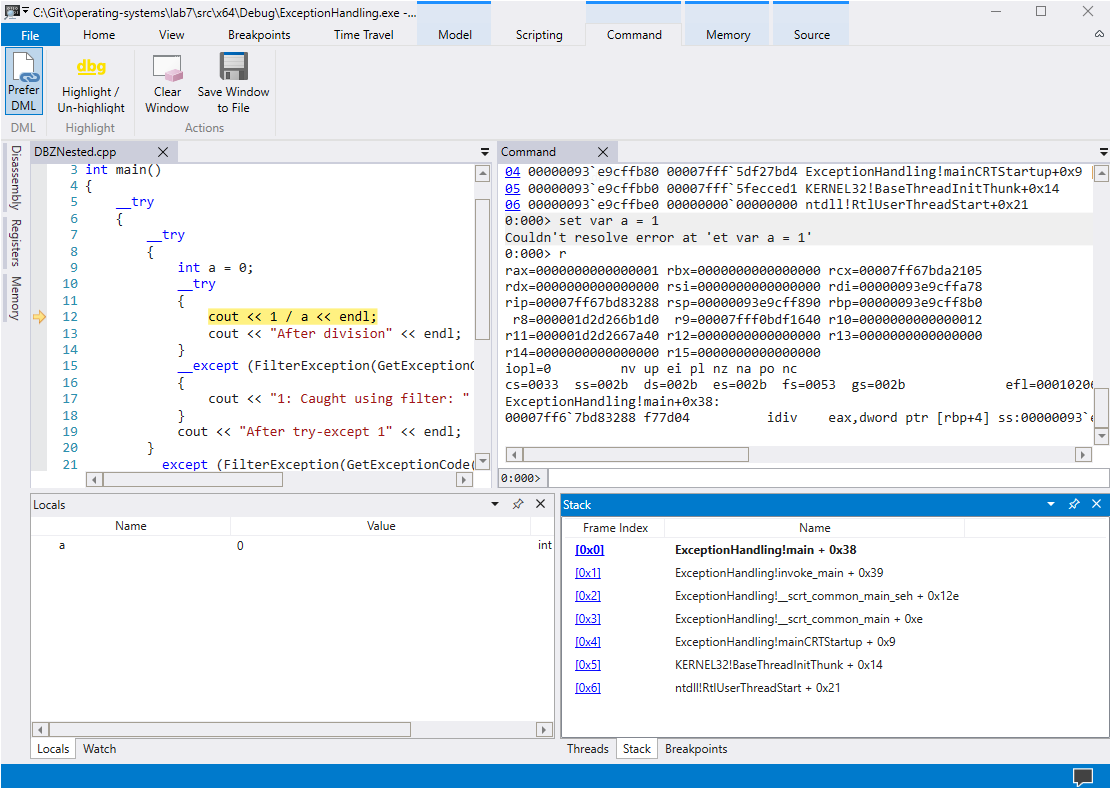
\includegraphics[width=\linewidth]{windbg}
	\caption{Графический интерфейс WinDbg}
	\label{fig:windbg}
\end{figure}

К основным командам интерактивной консоли WinDbg можно отнести:
\begin{itemize}[itemsep=-0.1cm]
	\item \code{.help} и \code{?} -- вывод доступных комманд;
	\item \code{.attach pid} -- подключиться к запущенному процессу;
	\item \code{.restart} -- перезапустить приложение;
	\item \code{ld module} -- загрузить символы для модуля \code{module};
	\item \code{g} -- продолжить выполнение программы;
	\item \code{p} -- запустить одну инструкцию, не заходя внутрь функций;
	\item \code{t} -- запустить одну инструкцию, зайдя внутрь функций;
	\item \code{pa addr} -- перейти по адресу \code{addr};
	\item \code{bp} -- установить точку останова;
	\item \code{bl} -- вывести список точек останова;
	\item \code{k} -- показать стек вызовов;
	\item \code{r} -- вывести содержимое регистров;
	\item \code{!analyze -v} -- вывести информацию о текущем исключении.
\end{itemize}

%Правильную работу с запускаемым приложением обеспечивает специальный файл program database \code{.pdb}. В нем содержится таблица соответствия адреса в памяти строке исходного кода программы и информация для анализа внутренней компоновки данных, используемых приложением. Интерфейс для работы с файлом \code{.pdb} предоставляют библиотеки \code{dbgHelp.dll} и \code{msDiaXY.dll}.

\newpage

\section{Выводы}

В процессе выполнения данной работы:

\begin{itemize}
	\item изучен механизм структурированной обработки исключений, свойственный ОС Windows;
	\item рассмотрены библиотечные функции для работы с исключениями;
	\item продемонстрирован порядок обработки необработанных исключений и вложенных блоков \code{__try};
	\item изучены способы досрочного завершения выполнения блока \code{__try} при помощи операторов \code{goto} и \code{__leave};
	\item рассмотрено использование финальных обработчиков \code{__finally} и их применимост в системных и прикладных программах.
	\item разработана программа для демонстрации результатов работы функции \code{AbnormalTermination()}.
\end{itemize}

\newpage

\section*{Список использованных источников}

\begin{enumerate}
	\item Душутина Е.В. -- Системное программное обеспечение. Практические вопросы разработки системных приложений [Текст] -- 2016.
	\item Таненбаум Э. -- Современные операционные системы [Текст] -- 2015.
	\item Structured Exception Handling / Microsoft Docs [Электронный ресурс]:\\
		{\small\url{https://docs.microsoft.com/en-us/cpp/cpp/structured-exception-handling-c-cpp}}
	\item Отладка программ с помощью WinDbg / Информационная безопаность на практике [Электронный ресурс]:\\
		{\small\url{http://www.spy-soft.net/debugging-using-windbg}}
	\item Common WinDbg Commands (Thematically Grouped) [Электронный ресурс]:\\
		{\small\url{http://windbg.info/doc/1-common-cmds.html}}
	\item \_\_ud2 / Microsoft Docs [Электронный ресурс]:\\
		{\small\url{https://docs.microsoft.com/en-us/cpp/intrinsics/ud2}}
	\item Microsoft-specific exception handling mechanisms / Википедия [Электронный ресурс]:\\
		{\small\url{https://en.wikipedia.org/wiki/Microsoft-specific_exception_handling_mechanisms}}
\end{enumerate}

\end{document}
